% Plantilla creada por Eduardo Mosqueira Rey
%
% Libro online bastante completo para consulta de Latex: http://en.wikibooks.org/wiki/LaTeX/
% Versión en castellano: http://es.wikibooks.org/wiki/Manual_de_LaTeX
\documentclass[12pt, a4paper, titlepage]{article}

\usepackage[spanish]{babel} % Soporte multilenguaje para LaTeX.

\usepackage[a4paper, top=2.5cm, bottom=2.5cm, left=2.5cm, right=2.5cm]{geometry} % Interfaz flexible para definir las dimensiones del documento

\usepackage[utf8]{inputenc} % Aceptar diferentes tipos de codificación de caracteres de entrada (en este caso usamos la codificación Unicode UTF-8)

\usepackage{graphicx} % Soporte aumentado para gráficos 
\usepackage{hyperref}
\begin{document}

%%%%%%%%%%%%%%%%%%%%%%%%%%%%%%%%%%%%%%%%%%%%%%%%%%%%%%%%%%%%%%%%%%%%%%%%%%%%%%%%
% PORTADA
%%%%%%%%%%%%%%%%%%%%%%%%%%%%%%%%%%%%%%%%%%%%%%%%%%%%%%%%%%%%%%%%%%%%%%%%%%%%%%%%

\begin{titlepage}


\includegraphics[width=15cm]{Imagenes/Simbolo_logo_UDC.png}

% Lista de tamaños: \Huge, \huge, \LARGE, \Large, \large, \small, \footnotesize, \tiny
\vspace{3cm}

\begin{center}

\includegraphics[scale=0.3]{Imagenes/1a_Practica_ER_14-15.png}
\end{center}


\begin{flushright}
	
	\LARGE{\textbf{ JoinMe!}}
	
	\LARGE{\textbf{Arquitectura lógica}}
	
	\large{\textbf{Version 1.0}}
	
\end{flushright}

\vspace{1cm}
\begin{center}
José Antonio López Sebio\\
Pablo Paz Varela\\
Grupo ER-12-03\\
\end{center}

\vspace{2cm}

\begin{center}
	\large{\textbf{Histórico}}
	
    \begin{tabular}{ | p{4cm} | p{2cm} | p{6cm} | p{3cm} |}
    \hline
    \textbf{Fecha} & \textbf{Version} & \textbf{Descripción} & \textbf{Autor} \\ \hline
      11/04/2014 & 1.0 & Primera Revisión & ER-12-03\\ \hline
      & 1.1 &  & ER-12-03\\ \hline
     &  & &\\ \hline
    \end{tabular}
\end{center}


\end{titlepage}
\clearpage

%%%%%%%%%%%%%%%%%%%%%%%%%%%%%%%%%%%%%%%%%%%%%%%%%%%%%%%%%%%%%%%%%%%%%%%%%%%%%%%%
% INDICE
%%%%%%%%%%%%%%%%%%%%%%%%%%%%%%%%%%%%%%%%%%%%%%%%%%%%%%%%%%%%%%%%%%%%%%%%%%%%%%%%

\tableofcontents
\clearpage

%%%%%%%%%%%%%%%%%%%%%%%%%%%%%%%%%%%%%%%%%%%%%%%%%%%%%%%%%%%%%%%%%%%%%%%%%%%%%%%%
\section{Introducción}
%%%%%%%%%%%%%%%%%%%%%%%%%%%%%%%%%%%%%%%%%%%%%%%%%%%%%%%%%%%%%%%%%%%%%%%%%%%%%%%%

%**********************************************************
\subsection{Propósito}
%**********************************************************

Este documento muestra una descripción del sistema usando diagramas y explicaciones textuales para representar la arquitectura lógica que está establecida en nuestro sistema.

%**********************************************************
\subsection{Alcance}
%**********************************************************

En este documento se especifica la organización en clases, paquetes, subsistemas y capas de la aplicación.

%**********************************************************
\subsection{Definiciones, Acrónimos y Abreviaturas}
%**********************************************************

Ver Glosario

%**********************************************************
\subsection{Referencias}
%**********************************************************

\begin{itemize}

    \item JoinMe! - Glosario
    \item JoinMe! - Modelo de casos de uso
    \item JoinMe! - Especificación suplementaria
    \item JoinMe! - Modelo del dominio
\end{itemize}

\pagebreak



%%%%%%%%%%%%%%%%%%%%%%%%%%%%%%%%%%%%%%%%%%%%%%%%%%%%%%%%%%%%%%%%%%%%%%%%%%%%%%%%
\section{Arquitectura lógica}
%%%%%%%%%%%%%%%%%%%%%%%%%%%%%%%%%%%%%%%%%%%%%%%%%%%%%%%%%%%%%%%%%%%%%%%%%%%%%%%%

\begin{center}
	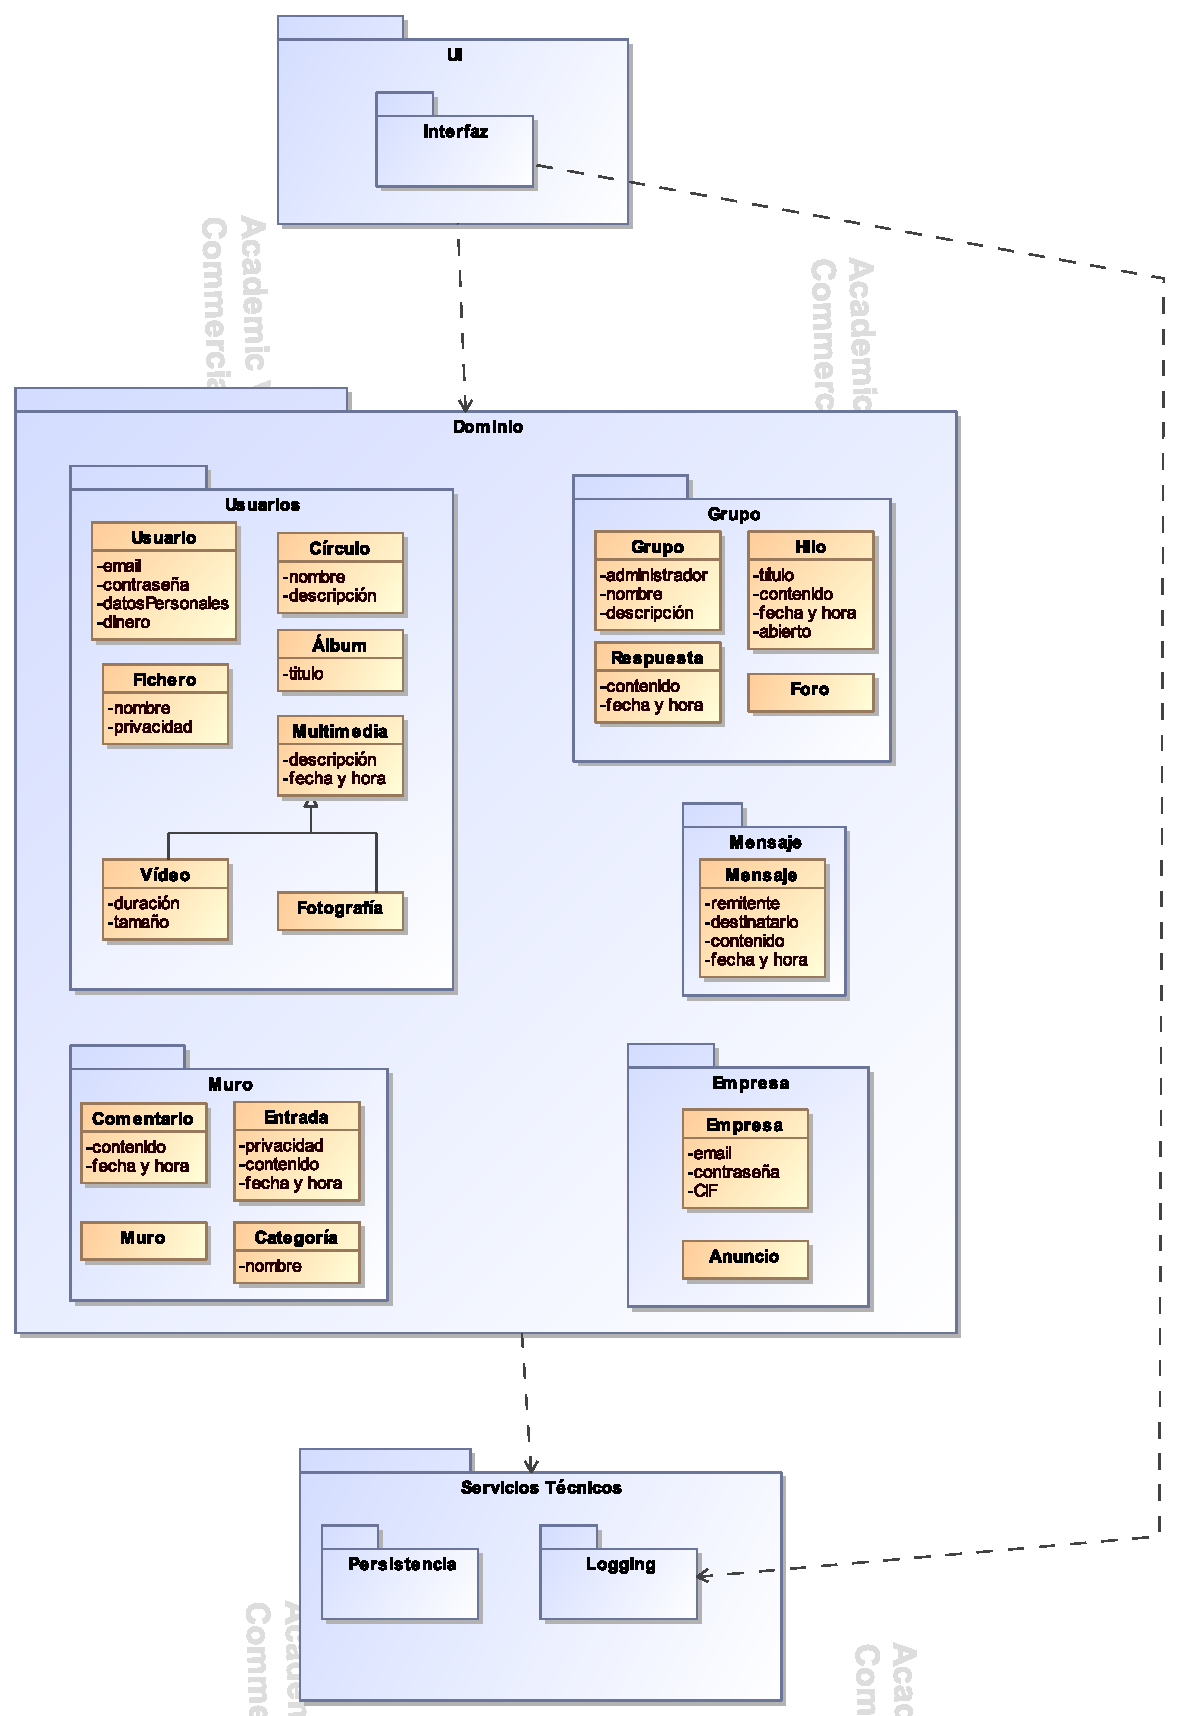
\includegraphics[width=\textwidth]{Imagenes/Arquitectura_logica}
\end{center}


\section{Explicación}

Considerando una división en tres capas:

\begin{itemize}
	\item \textbf{UI}: Capa que contiene el diseño de la interfaz de usuario para interactuar con el sistema.
	\item \textbf{Dominio}: Capa que contiene toda la lógica de negocio y las entidades que se emplean en el sistema.
	\item \textbf{Servicios Técnicos}: Capa donde se encuentra la persistencia de datos y el servicio de login de los usuarios.
\end{itemize}

\subsubsection{UI}
La interfaz de usuario es única, es decir, será la misma para navegadores de ordenadores, como para dispositivos móviles, ya que será una interfaz \textit{responsive} que se adaptará a las necesidades de cada pantalla. Por lo que sólo existe el paquete: 
	\begin{itemize}
		\item \textbf{Interfaz}: Inicialmente sea un usuario normal o una empresa no existiría diferencia ninguna. El usuario tendrá que hacer login para poder ver las opciones que tiene disponibles.
	\end{itemize}
	
	
\subsubsection{Dominio}

En la capa Dominio es donde se encuentra toda la lógica de negocio, en la cual hemos realizado la siguiente división por paquetes:
\begin{itemize}
	\item \textbf{Usuarios}: Contiene las clases relacionadas con los usuarios de la red social, tales como:
		\begin{itemize}
			\item Usuario
			\item Fichero
			\item Círculo
			\item Álbum
			\item Fichero
			\item Multimedia
			\item Vídeo
			\item Fotografía
		\end{itemize}
	\item \textbf{Muro}: Incluye las clases relacionadas directamente con el muro, como son: 
		\begin{itemize}
			\item Comentario
			\item Muro
			\item Entrada
			\item Categoría
		\end{itemize}
	\item \textbf{Grupo}: Clases relacionadas estrechamente con los Grupos.
		\begin{itemize}
			\item Grupo
			\item Foro
			\item Hilo
			\item Respuesta
		\end{itemize}
	\item \textbf{Empresa}: Agrupa las clases que representan a las empresas.
		\begin{itemize}
			\item Empresa
			\item Anuncio
		\end{itemize}
	
\end{itemize}


\subsubsection{Servicios Técnicos}

Este paquete contiene las clases relacionadas con los servicios técnicos:
\begin{itemize}
	\item \textbf{Persistencia}: Representa las clases y métodos que dan acceso a la base de datos con todos los datos de las redes sociales.
	\item \textbf{Login}: Servicio para comprobación de las credenciales de acceso a la red social.
\end{itemize}
\end{document}